\subsection{Operative's Turn Scenario}
Once a clue is given by a Spymaster, it is the Operative players turn to guess the cards on the board associated with that clue. In our system the GameManager calls an Operative object's makeMove, passing the given clue as a parameter. The Operative's play style is implemented using the Strategy design pattern. The Operative's makeMove method first telling its concrete strategy what the current clue is, and then by calling the OperativeStrategy's pickCard() class, passing the possible card choices as a parameter. The concrete strategy then returns one of the choices, and the Operative returns the choice to the GameManager.

\begin{figure}[H]
\centering
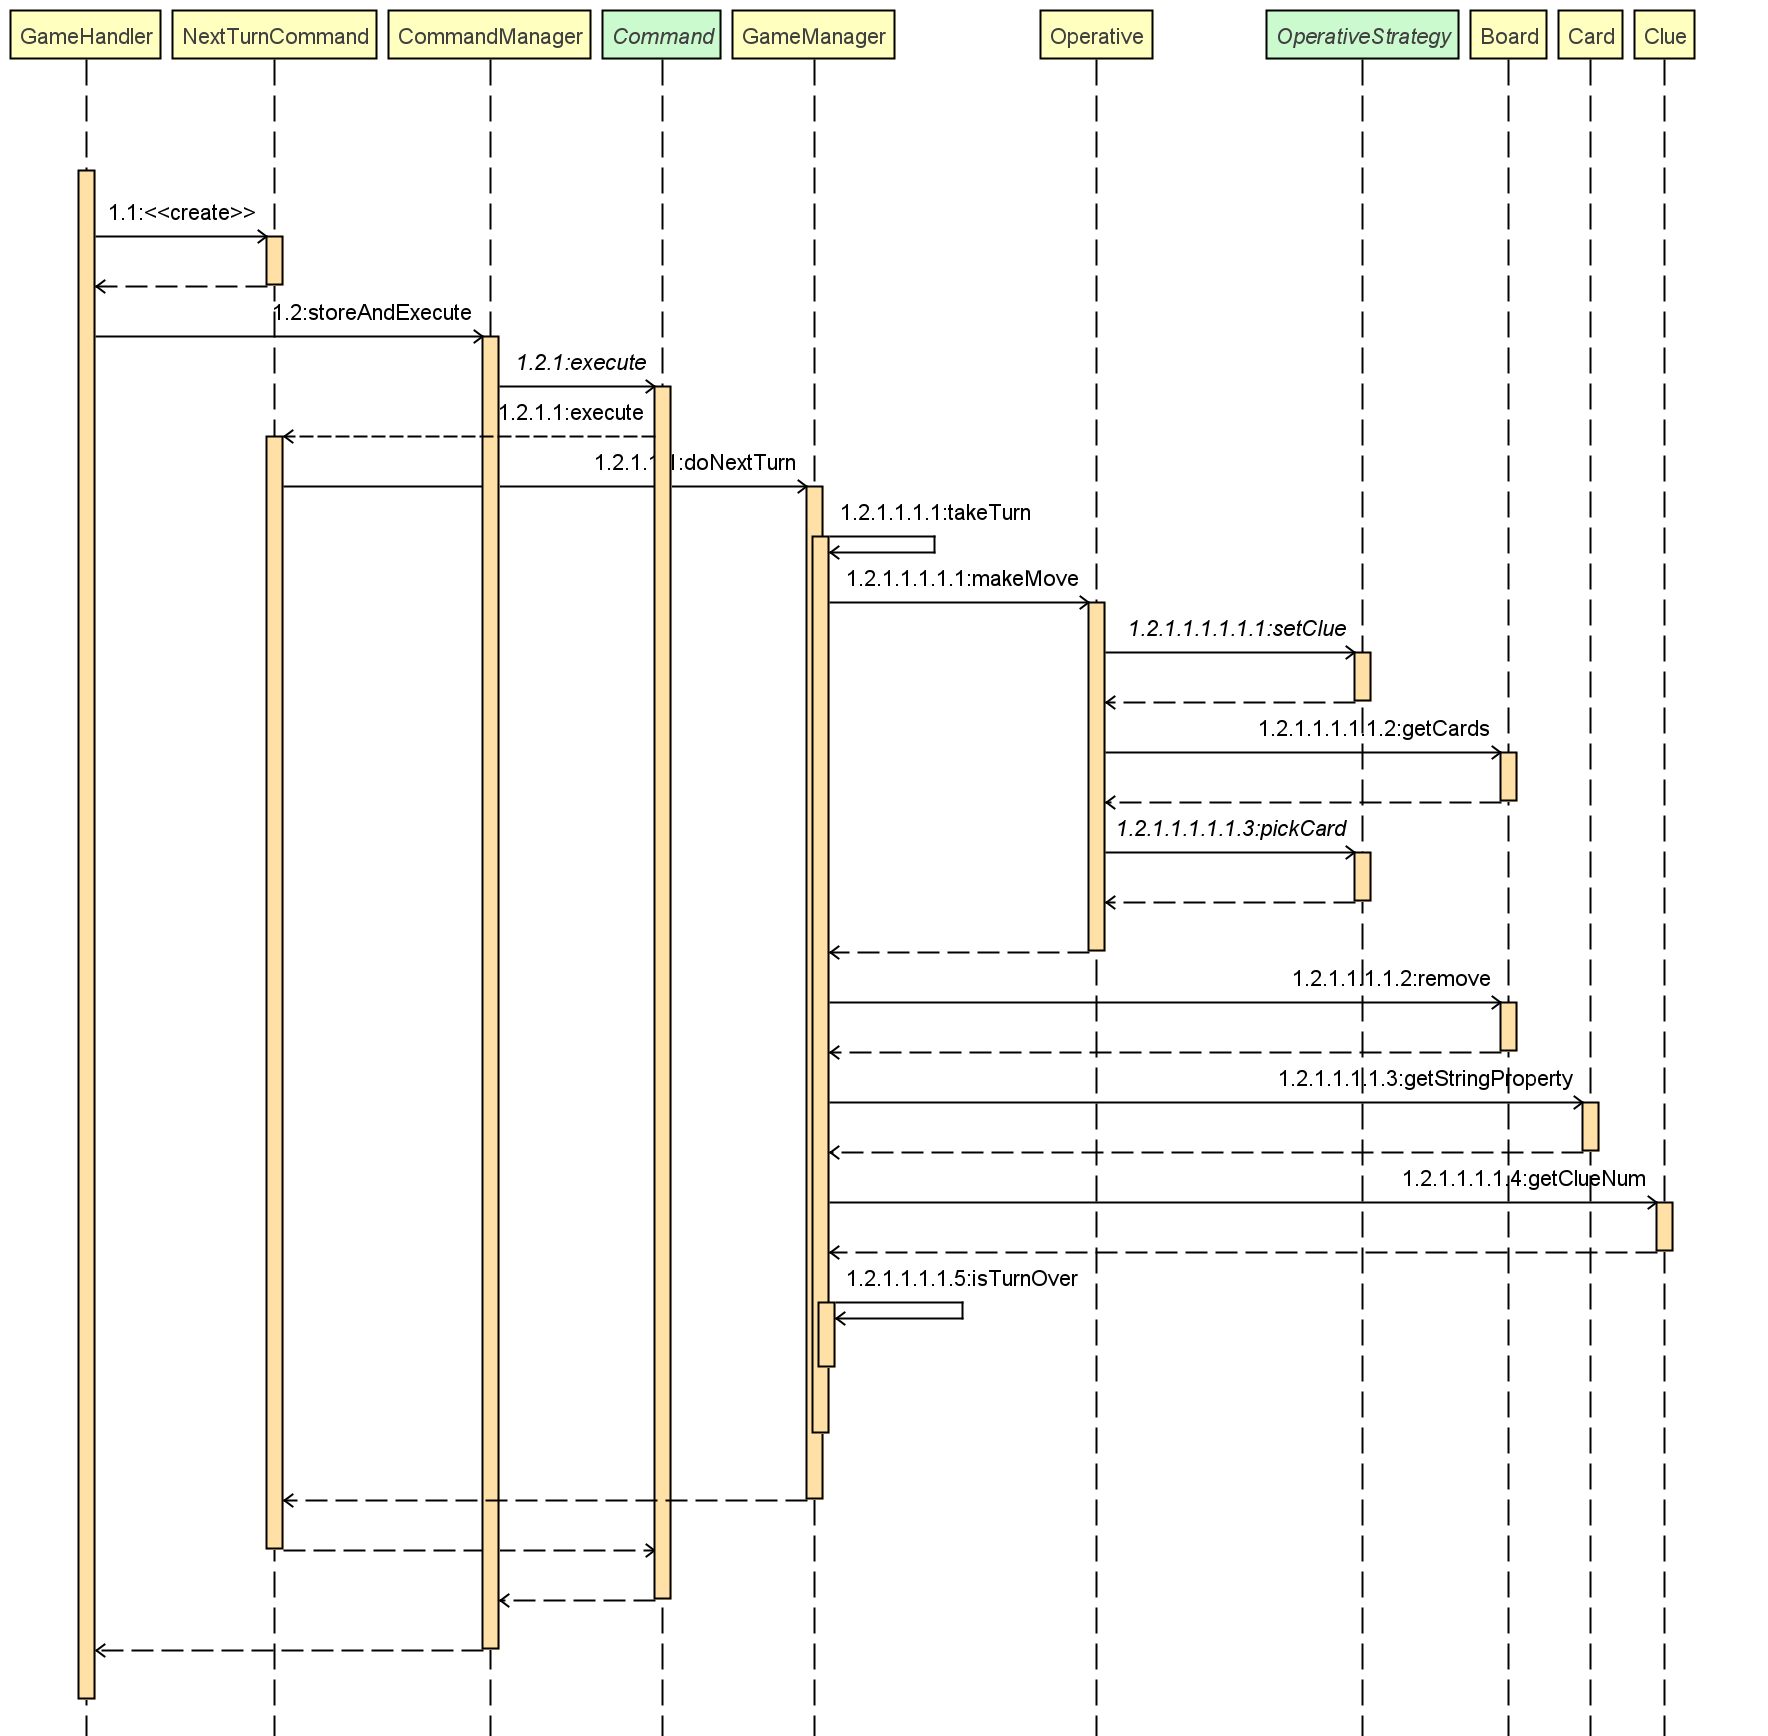
\includegraphics[width=10cm]{Source/DynamicDesign/Scenario/Operative.png}
\caption{Sequence Diagram of Operative}
\end{figure}